\chapter{Results} \label{chapResults}
\section{Quantitative evaluation}
\begin{itemize}
    \item Demonstrate that this planner does better than comparable batch planners in a head-to-head comparison
    \item Demonstrate that this planner does almost as well as online planners 
    \item Show the sensitivity to different algorithm configurations 
    \item Show the timing results, across different configurations
\end{itemize}

\section{Quantitative results}
\begin{itemize}
    \item The domain expert said this about our system 
    \item Here's the pretty result you get from our system
\end{itemize}

\begin{figure}
    \centering
    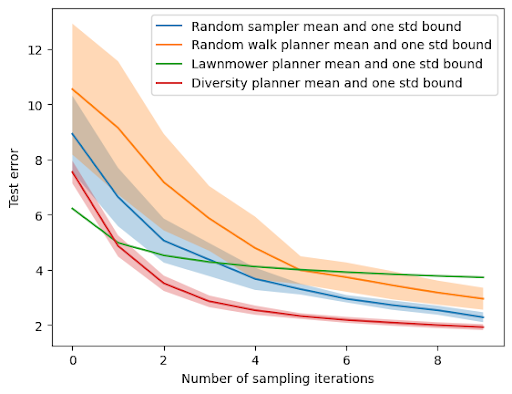
\includegraphics[width=\textwidth]{figs/results/GP_performance.png}
    \caption{This planner does better than everything else}
    \label{fig:quantitative}
\end{figure}

\begin{figure}
    \centering
    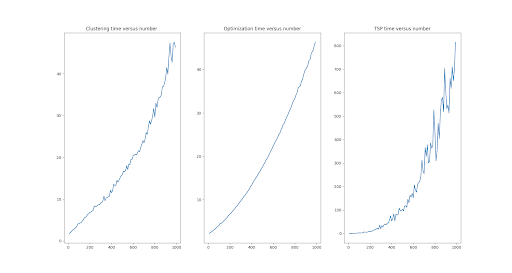
\includegraphics[width=\textwidth]{figs/results/timing.png}
    \caption{This is how long it takes to run each part}
    \label{fig:timing}
\end{figure}

\begin{figure}
    \centering
    \includegraphics[width=\textwidth]{example-image-a}
    \caption{Sensitivity analysis}
    \label{fig:sensetivity}
\end{figure}

\begin{figure}
    \centering
    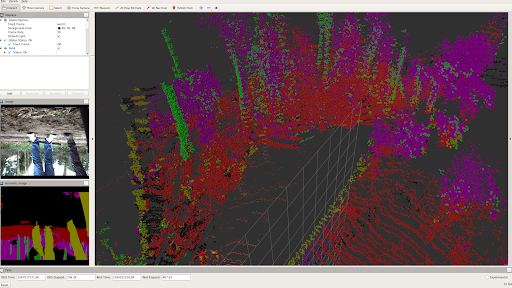
\includegraphics[width=\textwidth]{figs/results/semantic_mapping.png}
    \caption{You get this pretty thing when you run our system}
    \label{fig:pretty_thing}
\end{figure}